\documentclass[14pt]{article}
\usepackage[utf8]{inputenc}
\usepackage[T2A]{fontenc}
\usepackage[russian]{babel}
\usepackage{amsmath, amssymb}
\usepackage{geometry}
\usepackage{graphicx}
\usepackage{xcolor}
\usepackage{hyperref}
\usepackage{tasks}
\usepackage{tcolorbox}
\tcbuselibrary{skins, breakable}
\usepackage{fancyhdr}
\usepackage{lastpage}
\usepackage{enumitem}

% Настройка геометрии
\geometry{a4paper, left=20mm, right=15mm, top=25mm, bottom=25mm, headheight=20pt}

% Цвета
\definecolor{taskblue}{RGB}{0, 102, 204}
\definecolor{lightorange}{RGB}{255, 240, 220}
\pagecolor{lightorange!10}


\newtcolorbox[auto counter]{taskbox}[1][]{
  colback=white,
  colframe=taskblue,
  arc=5pt,
  boxrule=1.5pt,
  left=8pt,
  right=8pt,
  top=8pt,
  bottom=8pt,
  fonttitle=\bfseries\large,
  title=Задача \thetcbcounter,
  breakable,
  pad at break=2mm,
  #1
}
% Настройка tasks (варианты ответов в две колонки)
\settasks{
  label=\Alph*),
  label-width=1.8em,
  item-indent=2.5em,
  column-sep=2em,
  before-skip=3pt,
  after-skip=3pt
}

% Колонтитулы
\pagestyle{fancy}
\fancyhf{}
\fancyhead[L]{\textbf{MathCore} | MOCK Test-3}
\fancyhead[R]{Abdunazarov M.X.}
\fancyfoot[L]{\href{https://t.me/Math_Core_Dtm_MS_Att}{\textbf{MathCore}}}
\fancyfoot[R]{\href{https://t.me/Abd_mardon}{\textbf{@Abd\_mardon}}}
\fancyfoot[C]{\thepage/\pageref{LastPage}}
\renewcommand{\headrulewidth}{0.4pt}
\renewcommand{\footrulewidth}{0.4pt}

% Титульная страница
\title{\Huge \textbf{MOCK Test-3}}
\author{Abdunazarov M.X.}
\date{}

\begin{document}

\maketitle

\begin{center}
    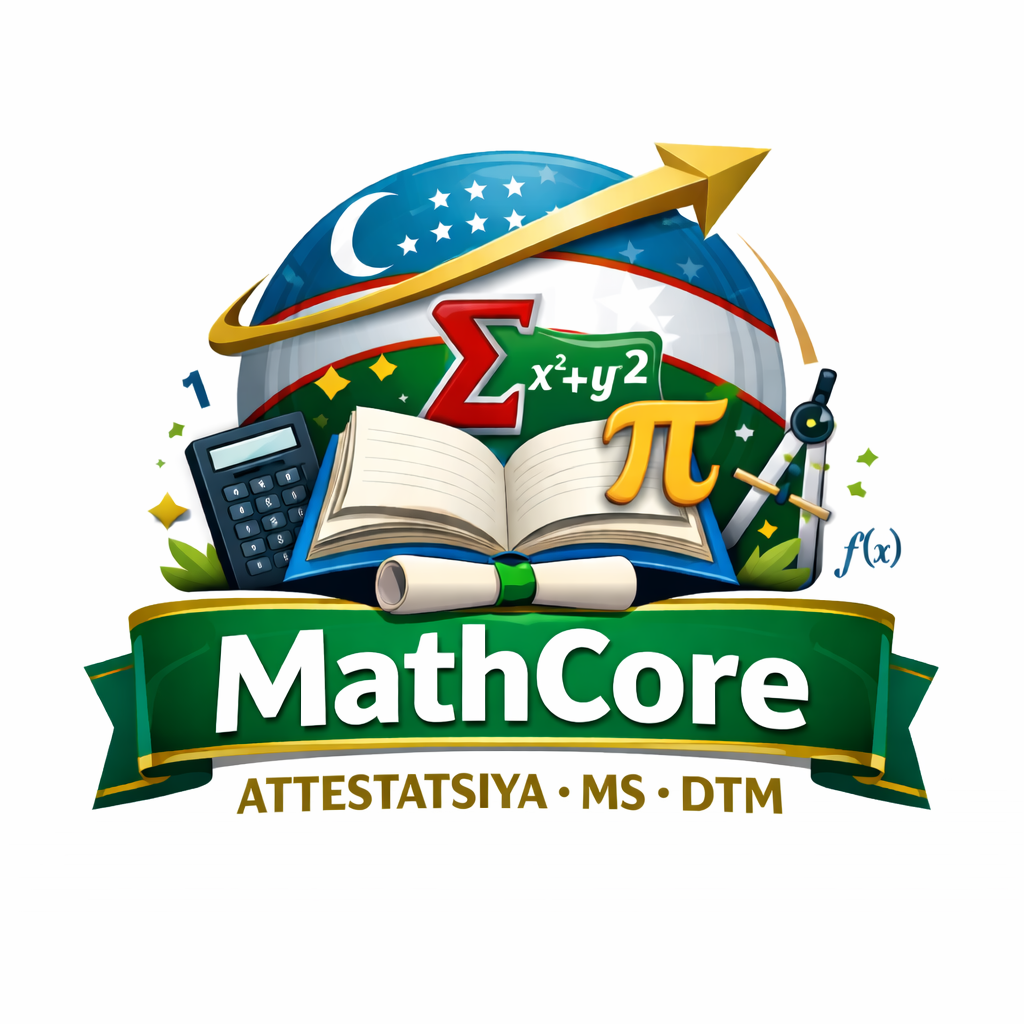
\includegraphics[width=0.3\textwidth]{logo.png}
\end{center}
\vspace{1cm}




\begin{taskbox}
При каком значении $a$ вершина параболы $y = x^2 - 2(a+1)x + 1$ находится ниже прямой $y = \frac{3}{4}$?
 \vspace{0.2cm} \begin{tasks}(2)
\task $(-\infty; -1) \cup (1; +\infty)$
\task $(-\frac{1}{2}; \frac{3}{2})$
\task $(-\infty; -\frac{3}{2}) \cup (-\frac{1}{2}; +\infty)$
\task $(-\infty; -\frac{1}{2}) \cup (\frac{3}{2}; +\infty)$
\end{tasks}
\vspace{2cm}
\end{taskbox}


\begin{taskbox}
Сколько натуральных делителей числа 210, не являющихся простыми?
 \vspace{0.2cm} \begin{tasks}(2)
\task 16
\task 15
\task 12
\task 11
\end{tasks}
\vspace{2cm}
\end{taskbox}

\begin{taskbox}
При каких значениях $a$ вершина параболы $y = ax^2 - x + a$ находится выше оси $Ox$?
 \vspace{0.2cm} \begin{tasks}(2)
\task $(-1; 0) \cup (1; +\infty)$
\task $(-\frac{1}{2}; 0) \cup (\frac{1}{2}; +\infty)$
\task $(-\infty; -\frac{1}{2}) \cup (\frac{1}{2}; +\infty)$
\task $(-\frac{1}{2}; 0)$
\end{tasks}
\vspace{2cm}
\end{taskbox}


\begin{taskbox}
Известно, что $\sin x = \frac{1}{3}$. Найдите значение выражения $\dfrac{\sin 2x - \sin 3x + \sin 5x}{1 + \cos x - 2\sin^2 2x}$.
 \vspace{0.2cm} \begin{tasks}(2)
\task $\frac{1}{2}$
\task $\frac{2}{5}$
\task $\frac{2}{3}$
\task $1$
\end{tasks}
\vspace{2cm}
\end{taskbox}


\begin{taskbox}
Решите неравенство $\arccos(3x - 4) < \arccos(x - 2)$.
 \vspace{0.2cm} \begin{tasks}(2)
\task $(1; +\infty)$
\task $(-1; 5/3]$
\task $[-1; 5/3]$
\task $(1; 5/3]$
\end{tasks}
\vspace{2cm}
\end{taskbox}

% Задача 36
\begin{taskbox}
При каких значениях параметра $a$ система уравнений $\begin{cases} 3x + ay - 13 = 0 \\ 2x - 3y + 5 = 0 \end{cases}$ имеет единственное решение?
 \vspace{0.2cm} \begin{tasks}(2)
\task $a \neq -4.5$
\task $a = -4.5$
\task $a = -6$
\task $a \neq -6$
\end{tasks}
\vspace{2cm}
\end{taskbox}


\begin{taskbox}
Сколько натуральных чисел, меньших 10, взаимно просты с 10?
 \vspace{0.2cm} \begin{tasks}(2)
\task 1
\task 2
\task 3
\task 4
\end{tasks}
\vspace{2cm}
\end{taskbox}


\begin{taskbox}
Найдите функцию, симметричную функции $y = -3^x + 5$ относительно точки $(2,7)$.
 \vspace{0.2cm} \begin{tasks}(2)
\task $y = 3^{x-4} + 9$
\task $y = 3^{-x+4} + 9$
\task $y = 3^{-x} - 5$
\task $y = 3^{x} - 5$
\end{tasks}
\vspace{2cm}
\end{taskbox}


\begin{taskbox}
В арифметической прогрессии $S_8 = 32$ и $S_{10} = 20$. Найдите $S_{18}$.
 \vspace{0.2cm} \begin{tasks}(2)
\task $-120$
\task $-115$
\task $-110$
\task $-108$
\end{tasks}
\vspace{2cm}
\end{taskbox}


\begin{taskbox}
Основания равнобедренной трапеции равны 22 и 42, а боковые стороны равны 26. Найдите её площадь.
 \vspace{0.2cm} \begin{tasks}(2)
\task 748
\task 768
\task 788
\task 808
\end{tasks}
\vspace{2cm}
\end{taskbox}


\begin{taskbox}
Площадь боковой поверхности конуса составляет 60\% от площади полной поверхности. Найдите отношение высоты конуса к радиусу основания.
 \vspace{0.2cm} \begin{tasks}(2)
\task $1.5$
\task $\frac{\sqrt{3}}{2}$
\task $\frac{\sqrt{5}}{2}$
\task $\frac{2}{3}$
\end{tasks}
\vspace{2cm}
\end{taskbox}


\begin{taskbox}
На боковых сторонах AB и CD трапеции ABCD взяты точки E и F так, что отрезки AF и ED пересекаются в точке O. Известно, что $BC:AD = 1:2$, $AE:AB = 1:2$, $FD:CD = 2:3$ и площадь трапеции равна 30. Найдите площадь треугольника AOE.
\begin{center}

\includegraphics[width=0.4\textwidth]{1.png}
\end{center}
 \vspace{0.2cm} \begin{tasks}(2)
\task 10
\task $\frac{5}{2}$
\task $\frac{20}{3}$
\task $\frac{10}{3}$
\end{tasks}
\vspace{2cm}
\end{taskbox}


\begin{taskbox}
Для равнобедренной трапеции ABCD, изображённой на рисунке, известно, что $CE:ED = 2:3$, $BC = 8$, $AD = 12$. Найдите отношение $S_{ABE}:S_{ADE}$.
\begin{center}

\includegraphics[width=0.4\textwidth]{2.png}
\end{center}
 \vspace{0.2cm} \begin{tasks}(2)
\task 5:4
\task 6:5
\task 4:3
\task 3:2
\end{tasks}
\vspace{2cm}
\end{taskbox}


\begin{taskbox}
В первом сосуде 5 годных и 5 бракованных деталей, во втором – 7 годных и 3 бракованных, в третьем – 8 годных и 2 бракованных. Найдите вероятность того, что случайно взятая деталь окажется годной и при этом из первого сосуда.
 \vspace{0.2cm} \begin{tasks}(2)
\task 0.21
\task 0.23
\task 0.2
\task 0.25
\end{tasks}
\vspace{2cm}
\end{taskbox}


\begin{taskbox}
Расстояние от дома до школы старший брат проходит за 24 минуты, а младший – за 30 минут. Если старший выйдет из дома на 3 минуты позже младшего, через сколько минут он догонит младшего?
 \vspace{0.2cm} \begin{tasks}(2)
\task 12
\task 15
\task 18
\task 24
\end{tasks}
\vspace{2cm}
\end{taskbox}


\begin{taskbox}
На стороне AB треугольника ABC взята точка D так, что $AD = 4$, $DB = 5$, $BC = 12$, $AC = 6$. Найдите длину отрезка CD.
\begin{center}

\includegraphics[width=0.4\textwidth]{3.png}
\end{center}
 \vspace{0.2cm} \begin{tasks}(2)
\task 6
\task 8
\task 7
\task 9
\end{tasks}
\vspace{2cm}
\end{taskbox}


\begin{taskbox}
Решите неравенство $\sin^2 x < \cos^2 x - \frac{\sqrt{3}}{2}$ на отрезке $[0; \pi]$.
 \vspace{0.2cm} \begin{tasks}(2)
\task $x \in [0; \frac{\pi}{12}) \cup (\frac{11\pi}{12}; \pi]$
\task $x \in [\frac{\pi}{12}; \frac{11\pi}{12}]$
\task $x \in [0; \frac{5\pi}{12})$
\task $x \in [0; \pi]$
\end{tasks}
\vspace{2cm}
\end{taskbox}


\begin{taskbox}
Имеются три сосуда. В первом 5 синих и 3 красных шара, во втором 4 синих и 4 красных, в третьем 5 красных и 3 синих. Наугад выбирают сосуд и из него извлекают один шар. Найдите вероятность того, что шар окажется красным.
 \vspace{0.2cm} \begin{tasks}(2)
\task $\frac{1}{4}$
\task $\frac{1}{3}$
\task $\frac{1}{2}$
\task $\frac{3}{4}$
\end{tasks}
\vspace{2cm}
\end{taskbox}


\begin{taskbox}
Найдите остаток от деления суммы $27^3 + 37^3$ на 13.
 \vspace{0.2cm} \begin{tasks}(2)
\task 6
\task 3
\task 5
\task 7
\end{tasks}
\vspace{2cm}
\end{taskbox}


\begin{taskbox}
Сумма коэффициентов разложения $(x + y)^n$ равна 4096. Найдите наибольший коэффициент многочлена.
 \vspace{0.2cm} \begin{tasks}(2)
\task 792
\task 864
\task 924
\task 936
\end{tasks}
\vspace{2cm}
\end{taskbox}


\begin{taskbox}
По данным на рисунке найдите площадь треугольника BDC.
\begin{center}

\includegraphics[width=0.4\textwidth]{4.png}
\end{center}
 \vspace{0.2cm} \begin{tasks}(2)
\task $18\sqrt{3}$
\task $16\sqrt{3}$
\task $15\sqrt{3}$
\task $24\sqrt{3}$
\end{tasks}
\vspace{2cm}
\end{taskbox}


\begin{taskbox}
Сколько целых чисел удовлетворяет неравенству $\sqrt{-x^2 + 6x - 4} > x - 4$?
 \vspace{0.2cm} \begin{tasks}(2)
\task 1
\task 2
\task 3
\task 4
\end{tasks}
\vspace{2cm}
\end{taskbox}


\begin{taskbox}
Вычислите $\sin 20^\circ \cdot \sin 40^\circ \cdot \sin 80^\circ$.
 \vspace{0.2cm} \begin{tasks}(2)
\task $\frac{\sqrt{3}}{4}$
\task $\frac{\sqrt{3}}{8}$
\task $\frac{\sqrt{3}}{16}$
\task $\frac{\sqrt{3}}{2}$
\end{tasks}
\vspace{2cm}
\end{taskbox}


\begin{taskbox}
Найдите объём тела, полученного вращением графика функции $y = -x^2 + 2x$ вокруг оси $Ox$.
 \vspace{0.2cm} \begin{tasks}(2)
\task $\frac{15\pi}{14}$
\task $\frac{17\pi}{16}$
\task $\frac{16\pi}{15}$
\task $\frac{13\pi}{12}$
\end{tasks}
\vspace{2cm}
\end{taskbox}


\begin{taskbox}
Сколькими способами можно выбрать 7 ручек, если имеются ручки 4 различных видов? (Ручки каждого вида считаются неразличимыми.)
 \vspace{0.2cm} \begin{tasks}(2)
\task 120
\task 56
\task 16384
\task 2401
\end{tasks}
\vspace{2cm}
\end{taskbox}


\begin{taskbox}
Найдите экстремумы функции:
\[
y = x^3 - 6x^2 + 9x + 5
\]
 \vspace{0.2cm} \begin{tasks}(2)
 \task Минимум при $x = 1$, максимум при $x = 3$
\task Минимум при $x = 3$, максимум при $x = 1$
\task Минимум при $x = 0$, максимум при $x = 2$
\taskНет экстремумов
 
\end{tasks}
\vspace{2cm}
\end{taskbox}


\begin{taskbox}
Найдите сумму корней уравнения $\sin 3x \cdot \cos 2x - \cos 3x \cdot \sin 2x = \frac{1}{2}$ на отрезке $[0; \pi]$.
 \vspace{0.2cm} \begin{tasks}(2)
\task $\pi$
\task $\frac{3\pi}{2}$
\task $\frac{2\pi}{3}$
\task нет корней
\end{tasks}
\vspace{2cm}
\end{taskbox}


\begin{taskbox}
Если $g(x) = x^3 f(x)$ – убывающая функция, то какое из неравенств выполняется всегда?
 \vspace{0.2cm} \begin{tasks}(2)
\task $f(x) > f'(x)$
\task $x f'(x) < -3f(x)$
\task $f'(x) > f(x)$
\task $x^2 f(x) > x f'(x)$
\end{tasks}
\vspace{2cm}
\end{taskbox}


\begin{taskbox}
На рисунке изображены графики функций $y = 2x^2$ и $y = 4 - x$. Найдите максимальное значение площади прямоугольника, вписанного в область между ними.
\begin{center}

\includegraphics[width=0.4\textwidth]{6.png}
\end{center}
 \vspace{0.2cm} \begin{tasks}(2)
\task $\frac{35}{22}$
\task $\frac{44}{27}$
\task $\frac{47}{26}$
\task $\frac{49}{35}$
\end{tasks}
\vspace{2cm}
\end{taskbox}


\begin{taskbox}
В школьной столовой есть 4 вида сладостей. Сколькими способами ученик может выбрать 5 сладостей? (Порядок не важен, сладости одного вида неразличимы.)
 \vspace{0.2cm} \begin{tasks}(2)
\task 1024
\task 625
\task 56
\task 120
\end{tasks}
\vspace{2cm}
\end{taskbox}


\begin{taskbox}
Найдите все решения уравнения:
\[
2\sin^2 x - 3\sin x + 1 = 0, \quad x \in [0, 2\pi].
\]

 \vspace{0.2cm} \begin{tasks}(2)
\task  $x = \frac{\pi}{6}, \frac{5\pi}{6}$
\task $x = \frac{\pi}{4}, \frac{3\pi}{4}$
\task $x = \frac{\pi}{3}, \frac{2\pi}{3}$
\task $x = 0, \pi$
\end{tasks}
\vspace{2cm}
\end{taskbox}


\begin{taskbox}
Из прямоугольника $ABCD$ вырезали треугольник $ECD$. $AB = 6$, $AD = ED$. Найдите площадь четырехугольника $ABED$, если она максимальна.
\begin{center}

\includegraphics[width=0.4\textwidth]{8.png}
\end{center}
 \vspace{0.2cm} \begin{tasks}(2)
\task $18\sqrt{3}$
\task $16\sqrt{3}$
\task $14\sqrt{3}$
\task $12\sqrt{3}$
\end{tasks}
\vspace{2cm}
\end{taskbox}


\begin{taskbox}
Если $a \parallel b$, найдите угол $\alpha$.
\begin{center}

\includegraphics[width=0.4\textwidth]{9.png}
\end{center}
 \vspace{0.2cm} \begin{tasks}(2)
\task $140^\circ$
\task $160^\circ$
\task $150^\circ$
\task $120^\circ$
\end{tasks}
\vspace{2cm}
\end{taskbox}


\begin{taskbox}
Найдите радиус окружности, вписанной в прямоугольный треугольник.
\begin{center}
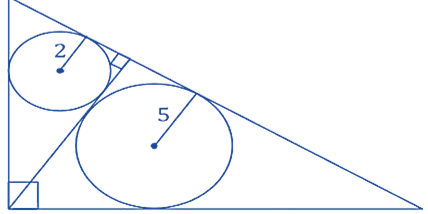
\includegraphics[width=0.4\textwidth]{10.png}
\end{center}
 \vspace{0.2cm} \begin{tasks}(2)
\task 3
\task 7
\task $\sqrt{29}$
\task $\sqrt{21}$
\end{tasks}
\vspace{2cm}
\end{taskbox}


\begin{taskbox}
Расстояние между городами $A$ и $B$ равно 120 км. Поезд сделал остановку на 10 минут в середине пути и продолжил движение со скоростью на 12 км/ч больше первоначальной. Весь путь занял 2 часа 25 минут (включая остановку).Найдите первоначальную скорость поезда (в км/ч).
\vspace{0.2cm} \begin{tasks}(2)
\task 45
\task 52
\task 44
\task 48
\end{tasks}
\vspace{2cm}
\end{taskbox}



\end{document}